\section{Tidsplan}

Til planlægningen af projekt blev der lavet en tidsplan i starten af projektet. Tidsplanen blev derefter justeret efter prioritering og deadlines. Tidsplanen er inddelt i to dele: udformning af produkt og fremstillingen af dokumentation- og rapportskrivning.

\begin{figure}[H]
    \centering
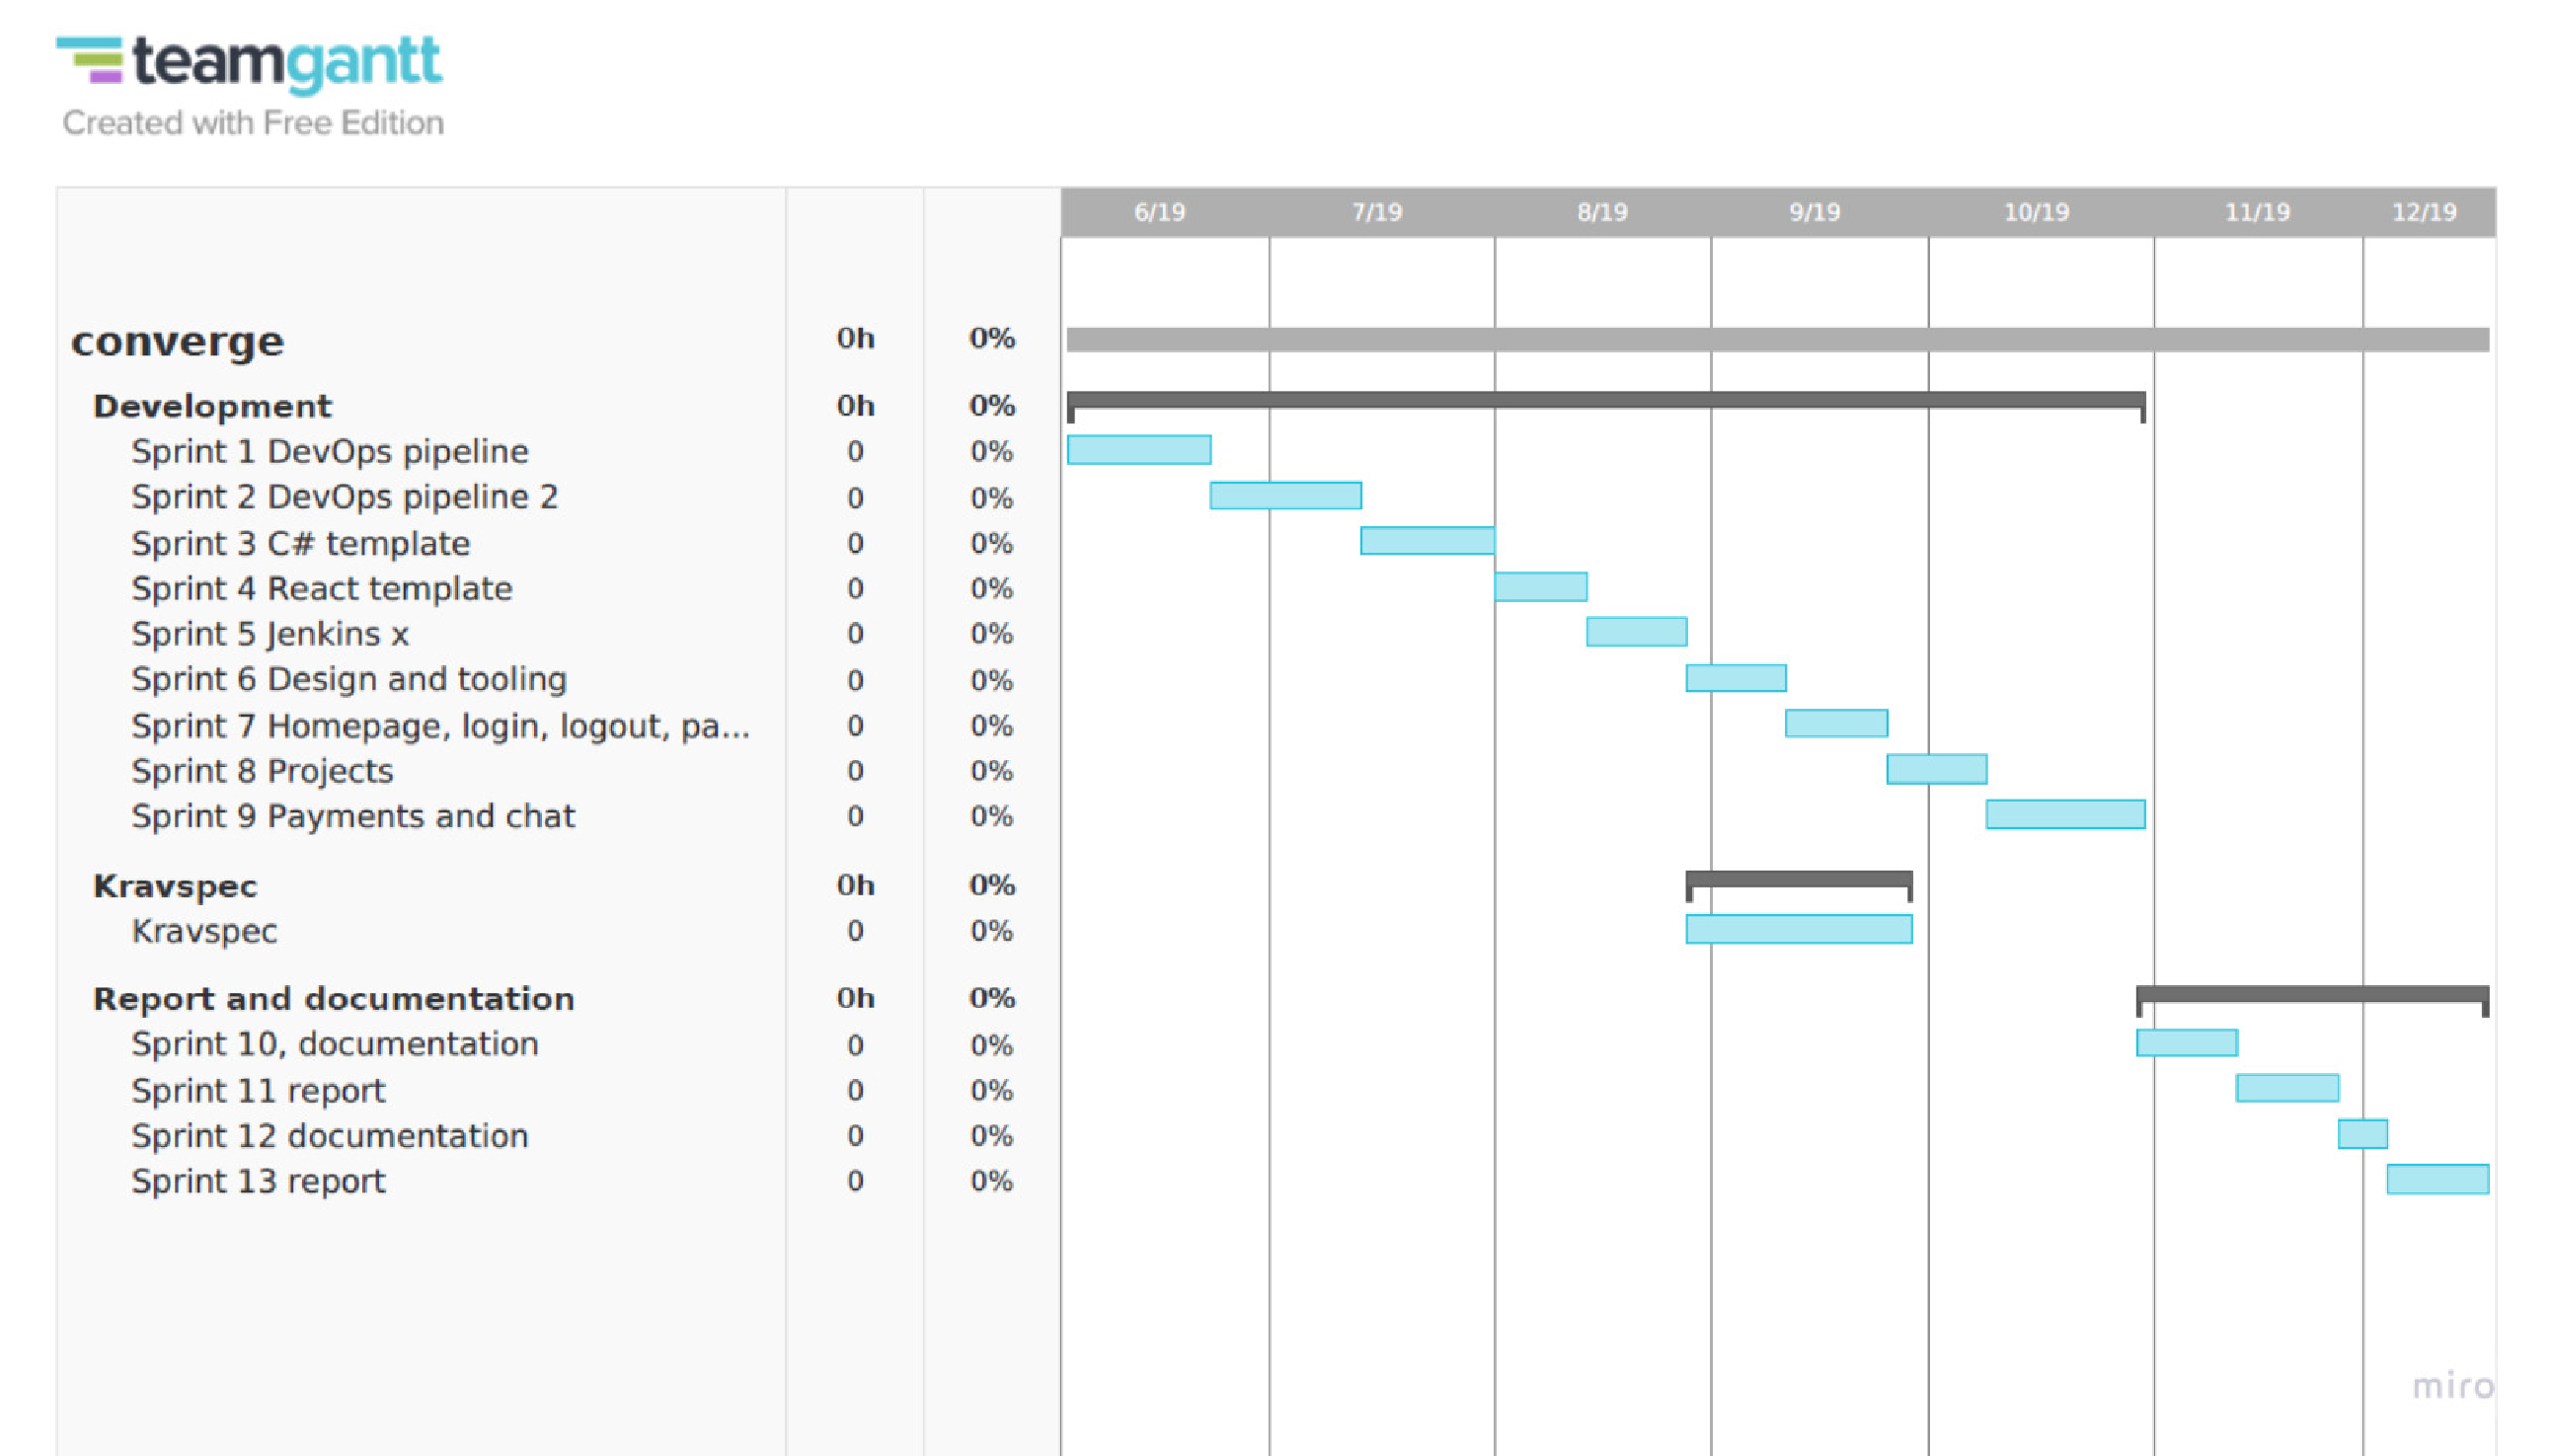
\includegraphics[width=0.7\textwidth]{Billeder/schedule1.pdf}
\caption{Viser et oversigt over tidsplanen}
\label{fig:figure4}
\end{figure}
\newpage
\section{Roadmap}

Roadmap er en plan over hvor langt de forskellige Epics er, fra være færdige, dette er ikke det samme som tidsplanen, men viser det resterende arbejde tilbage for de forskellige parter.


\begin{figure}[H]
    \centering
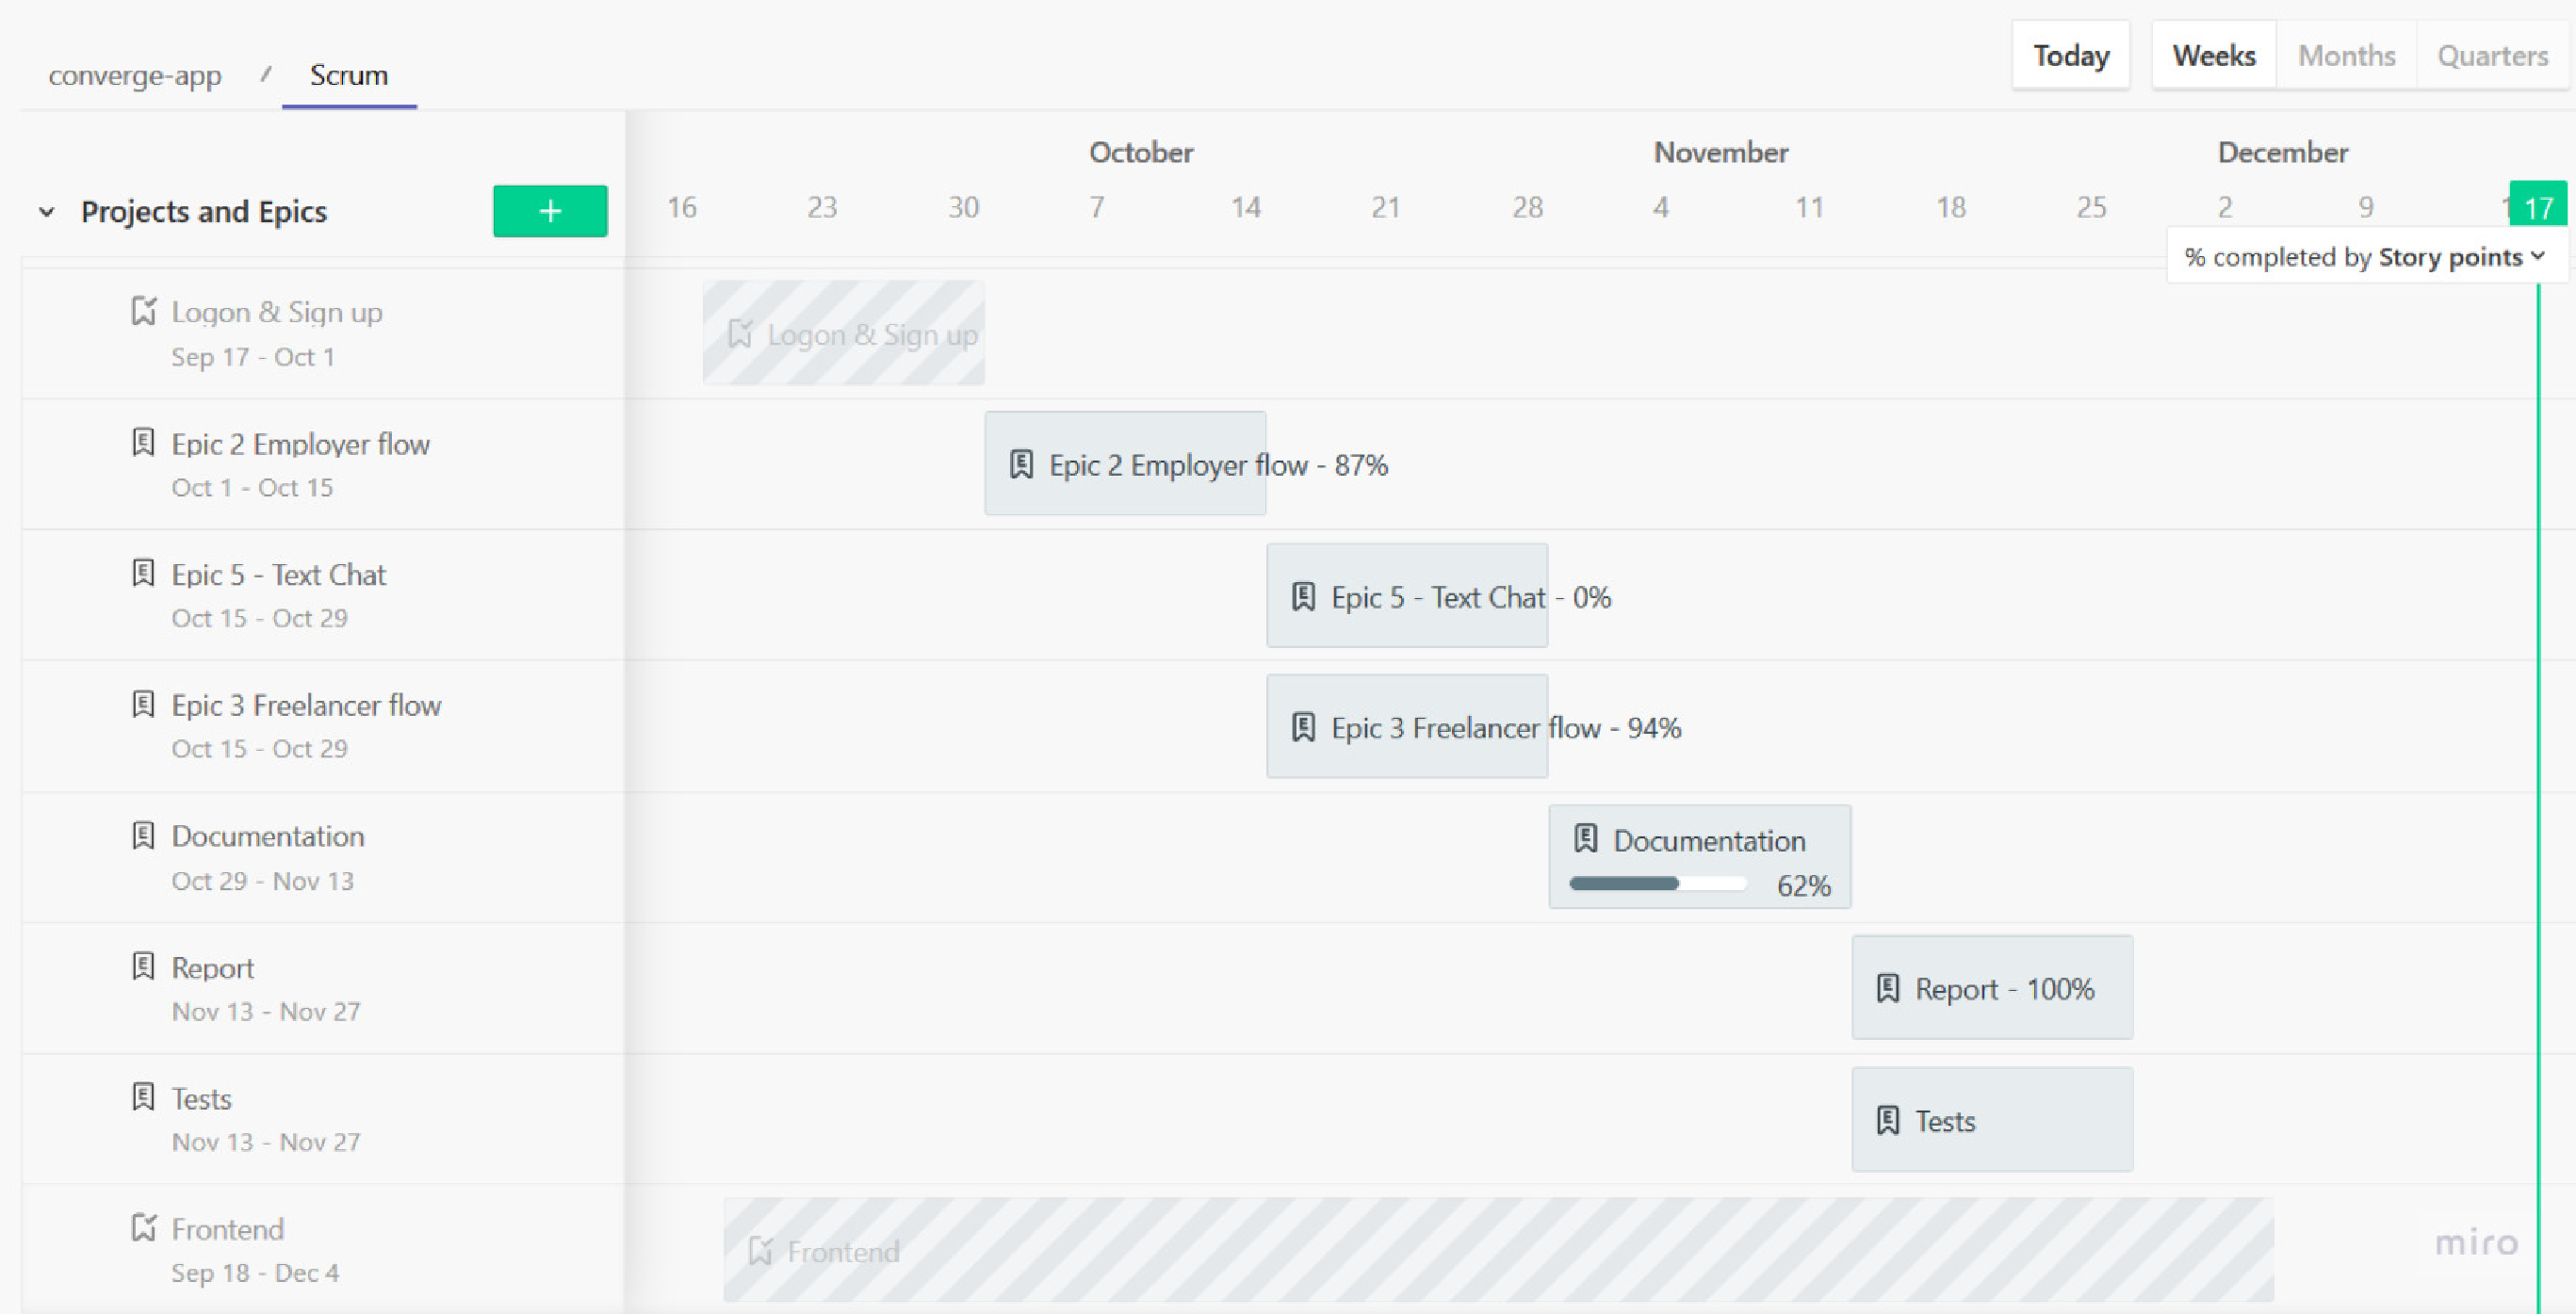
\includegraphics[width=0.7\textwidth]{Billeder/roadmap.pdf}
\caption{Viser Roadmap over forskellige Epics}
\label{fig:figure4}
\end{figure}
